179. \begin{figure}[ht!]
\center{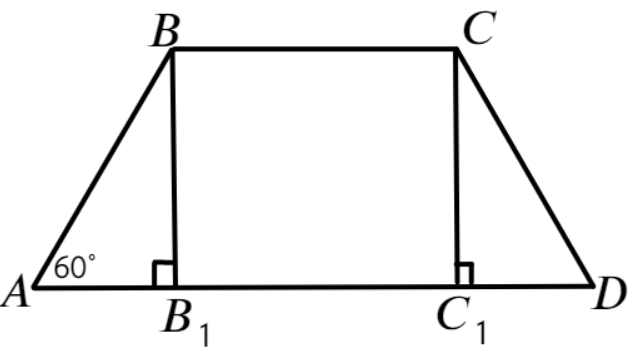
\includegraphics[scale=0.35]{g8-179.png}}
\end{figure}\\
Опустим высоты $BB_1$ и $CC_1.$ Так как трапеция равнобедренная, $AB_1=C_1D=(12-6):2=3$см. Тогда $BB_1=AB_1\ tg(60^\circ)=3\sqrt{3}$см. Таким образом, $S_{ABCD}=3\sqrt{3}\cdot\cfrac{12+6}{2}=27\sqrt{3}\text{ см}^2.$\\
